\documentclass[12pt,a4paper]{article}

% Pacotes necessários
\usepackage[utf8]{inputenc}
\usepackage[portuguese]{babel}
\usepackage[T1]{fontenc}
\usepackage{amsmath}
\usepackage{amsfonts}
\usepackage{amssymb}
\usepackage{graphicx}
\usepackage{float}
\usepackage{caption}
\usepackage{subcaption}
\usepackage{geometry}
\usepackage{setspace}
\usepackage{indentfirst}
\usepackage{listings}
\usepackage{xcolor}
\usepackage{hyperref}
\usepackage{booktabs}
\usepackage{array}
\usepackage{multirow}
\usepackage{fancyhdr}
\usepackage{verbatim}

% Configurações da página
\geometry{left=3cm,right=2cm,top=3cm,bottom=2cm}
\setlength{\headheight}{14pt}
\onehalfspacing

% Configurações do hyperref
\hypersetup{
    colorlinks=true,
    linkcolor=black,      
    filecolor=magenta,      
    urlcolor=blue,
    citecolor=black,
}

% Configuração do cabeçalho
\pagestyle{fancy}
\fancyhf{}
\fancyhead[L]{\small Trabalho 02 - Árvores Binárias}
\fancyhead[R]{\small \thepage}
\renewcommand{\headrulewidth}{0.4pt}

% Configuração para código
\lstset{
    language=Python,
    basicstyle=\footnotesize\ttfamily,
    keywordstyle=\color{blue}\bfseries,
    commentstyle=\color{green!60!black},
    stringstyle=\color{red},
    numbers=left,
    numberstyle=\tiny\color{gray},
    stepnumber=1,
    numbersep=5pt,
    backgroundcolor=\color{gray!10},
    frame=single,
    breaklines=true,
    breakatwhitespace=true,
    captionpos=b
}


\begin{document}
\begin{titlepage}
    \begin{center}
        \vspace*{2cm}
        \textbf{CENTRO FEDERAL DE EDUCAÇÃO TECNOLÓGICA DE MINAS GERAIS} \\[1.5cm]
        \textbf{PÓS-GRADUAÇÃO EM CIÊNCIA DA COMPUTAÇÃO} \\[4cm]
        \textbf{ALGORTIMOS E ESTRUTURAS DE DADOS} \\[0.5cm]
        \large{Comparação entre Árvores Binárias de Pesquisa e Árvores AVL} \\[0.5cm]
        \large{Análise de Desempenho em Operações de Busca} \\[4cm]
        \textbf{Leonardo Vieira Guimarães} \\[2cm]
        Belo Horizonte \\[0.5cm]
        \the\year
    \end{center}
\end{titlepage}


\begin{abstract}
Este trabalho compara, de forma simples e prática, duas estruturas muito usadas para busca de dados: a Árvore Binária de Pesquisa (BST) e a Árvore AVL. A BST é fácil de entender, mas pode ficar lenta se os dados forem inseridos em ordem. Já a AVL se ajusta automaticamente, mantendo sempre a busca rápida, mesmo com dados ordenados. Foram realizados experimentos com diferentes tamanhos de árvore (de 1.000 a 10.000 elementos) e dois tipos de inserção: ordenada e aleatória. Os resultados mostram que a AVL garante eficiência em todos os casos, enquanto a BST só é eficiente com dados aleatórios. Assim, o estudo reforça a importância do balanceamento automático para manter a velocidade das buscas.

\textbf{Palavras-chave:} BST, AVL, Estruturas de Dados, Busca, Complexidade, Algoritmos.
\end{abstract}

\newpage
\tableofcontents
\newpage

\section{Introdução}



\textbf{Árvore Binária de Pesquisa (BST):} Estrutura onde cada nó possui até dois filhos, sendo o da esquerda menor e o da direita maior que o valor do nó. Permite buscas rápidas quando está balanceada, pois a cada comparação metade dos valores é descartada. Porém, se os dados forem inseridos em ordem crescente ou decrescente, a BST pode se degenerar em uma lista ligada, tornando as buscas lentas (complexidade O(n)). É fácil de implementar e funciona bem com dados aleatórios, mas não garante sempre a melhor performance.

\textbf{Árvore AVL:} Variante da BST que se auto-balanceia após cada inserção ou remoção. Monitora a diferença de altura entre os lados da árvore e realiza rotações automáticas para manter o equilíbrio. Isso garante que a altura permaneça próxima ao logaritmo do número de elementos, mantendo buscas, inserções e remoções sempre rápidas (complexidade O(log n)), independentemente da ordem dos dados. A implementação é mais complexa, mas oferece desempenho previsível e robusto, ideal para aplicações que exigem eficiência constante.

Essas duas estruturas são amplamente discutidas em literatura clássica, como em Cormen et al. (2009)\cite{cormen2009}, que detalham suas características, funcionamento e diferenças de desempenho.

As árvores binárias de pesquisa (BST) e as árvores AVL são estruturas fundamentais em ciência da computação, especialmente para operações de busca, inserção e remoção em grandes conjuntos de dados. A BST é simples e eficiente quando os dados são inseridos de forma aleatória, mas pode apresentar desempenho linear (O(n)) se os dados forem inseridos em ordem, degenerando em uma lista ligada. Já a AVL é uma BST auto-balanceada, que garante altura logarítmica e desempenho consistente (O(log n)) independentemente da ordem de inserção, graças ao balanceamento automático por rotações.

Este trabalho investiga, de forma prática e didática, as diferenças de desempenho entre BSTs sem balanceamento e árvores AVL, considerando diferentes padrões de inserção de dados. O objetivo é demonstrar empiricamente como o balanceamento influencia a eficiência das operações de busca e orientar a escolha adequada de estruturas em projetos de software.

\section{Metodologia}

\subsection*{Justificativa dos Parâmetros}
Para garantir resultados confiáveis e reduzir o impacto de variações aleatórias, cada experimento foi repetido com 10 árvores diferentes para cada configuração. O valor de n (tamanho da árvore) variou de 1.000 a 10.000 elementos, permitindo observar o comportamento das estruturas tanto em cenários pequenos quanto em grandes volumes de dados. Essa abordagem proporciona uma análise mais robusta e representativa dos algoritmos.

Esta seção descreve detalhadamente o processo experimental adotado para comparar o desempenho das estruturas BST e AVL. Foram definidos procedimentos claros para garantir a reprodutibilidade dos resultados e a análise objetiva dos dados obtidos.

\subsection*{Passos Realizados}
\begin{itemize}
    \item Desenvolver e testar as implementações das estruturas BST e AVL em Python, garantindo contagem de comparações nas buscas.
    \item Preparar o ambiente computacional com Jupyter Notebook, utilizando as bibliotecas NumPy para manipulação de dados e Matplotlib para geração dos gráficos.
    \item Definir os tamanhos das árvores para os testes: de 1.000 até 10.000 elementos, em intervalos regulares.
    \item Realizar 10 repetições para cada configuração, aumentando a confiabilidade dos resultados.
    \item Executar experimentos em dois cenários distintos:
    \begin{itemize}
        \item Inserção ordenada dos elementos (simulando o pior caso para BST)
        \item Inserção aleatória dos elementos (simulando o caso médio)
    \end{itemize}
    \item Realizar buscas pelo elemento 10.001, que não está presente nas árvores, para garantir avaliação do pior caso de busca.
    \item Registrar e organizar os resultados obtidos em cada cenário experimental.
    \item Analisar os dados coletados e construir gráficos comparativos para facilitar a interpretação dos resultados.
\end{itemize}

\subsection*{Métricas Utilizadas}
\begin{itemize}
    \item \textbf{Número de comparações na busca}: Quantifica o esforço computacional para localizar um elemento, sendo o principal indicador de eficiência das estruturas.
    \item \textbf{Complexidade teórica}: Utilização dos limites O(n) e O(log n) para comparar o comportamento prático com o esperado pela teoria.
    \item \textbf{Média das repetições}: Avaliação da consistência dos resultados, reduzindo o impacto de variações aleatórias.
    \item \textbf{Influência do padrão de inserção}: Comparação entre cenários ordenados e aleatórios para identificar o impacto do balanceamento na performance.
\end{itemize}

\section{Resultado e Discussão}


A seguir, são apresentados e explicados os principais gráficos do trabalho, ilustrando o comportamento das estruturas em diferentes cenários. Cada gráfico está referenciado e acompanhado de uma explicação detalhada sobre o que representa.


\subsection*{BST com Inserções Ordenadas}
\begin{figure}[H]
    \centering
    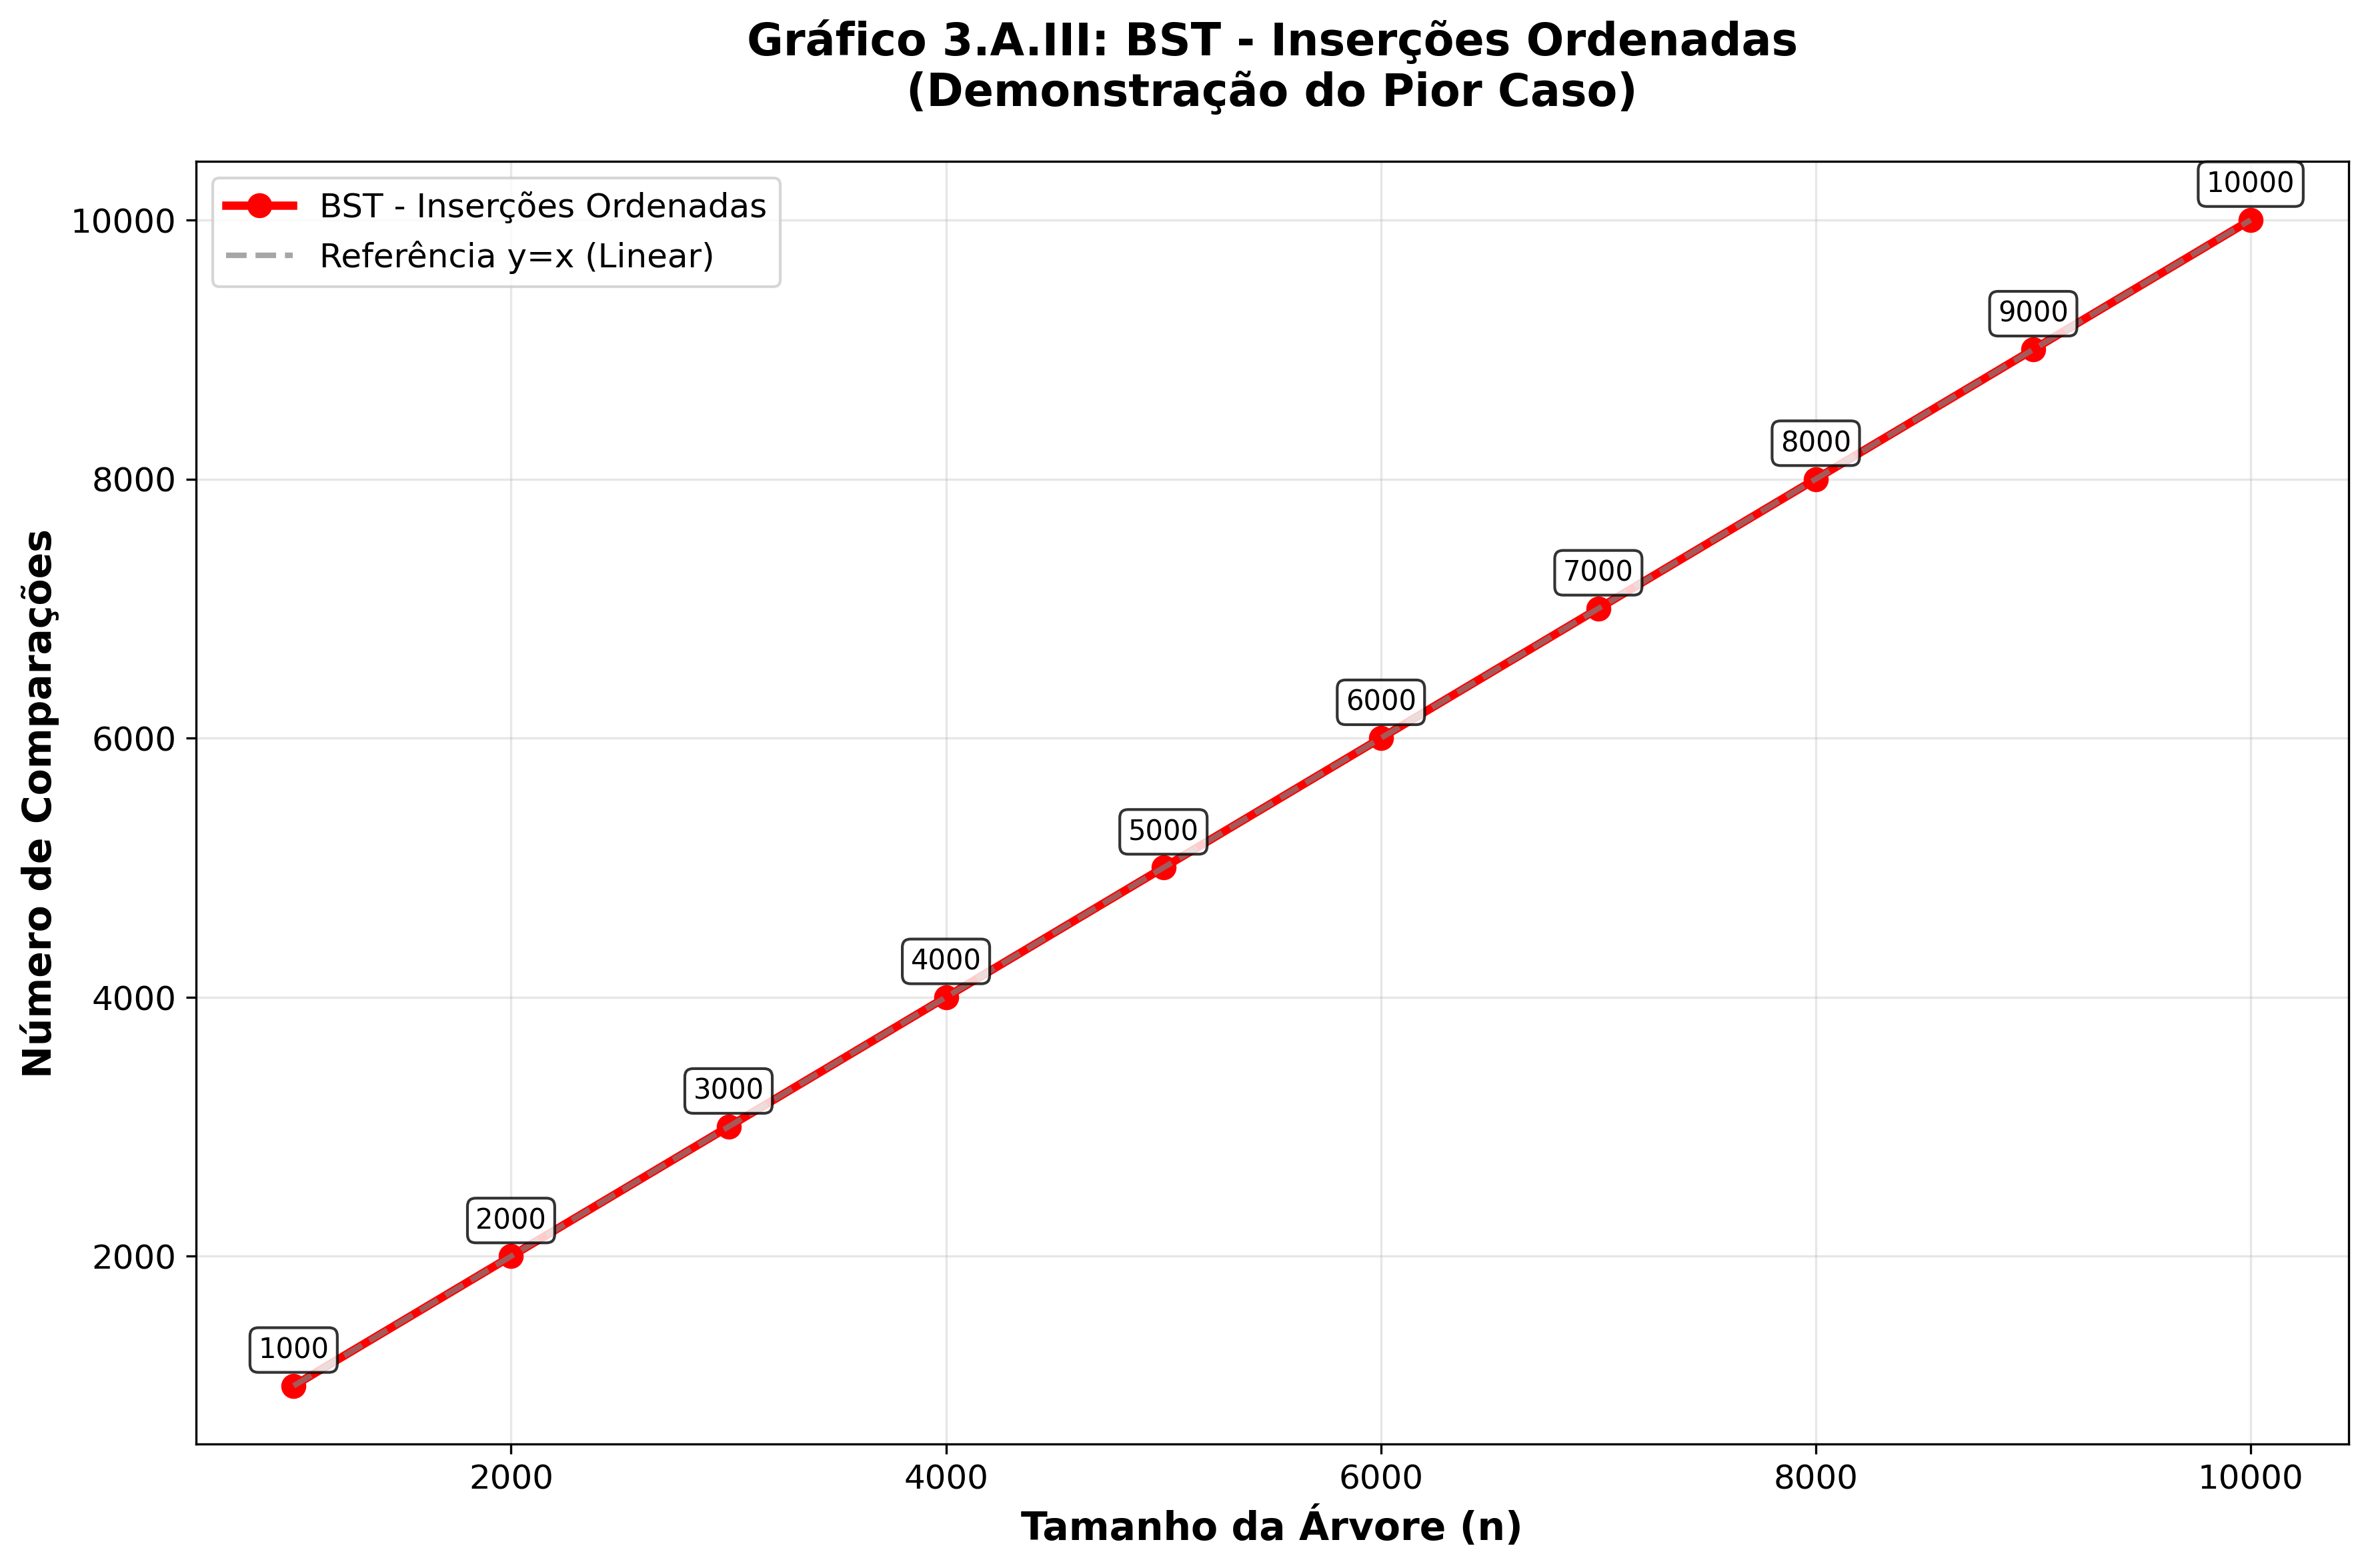
\includegraphics[width=0.8\textwidth]{graficos/grafico_3A_III_bst_ordenados.png}
    \caption{Gráfico 3.A.III: BST - Inserções Ordenadas (Demonstração do Pior Caso)}
    \label{fig:bst_ordenados}
\end{figure}
Como podemos ver no gráfico da Figura~\ref{fig:bst_ordenados}, quando inserimos dados em ordem na BST, ela vira uma "escada". Cada busca precisa passar por todos os nós, então quanto maior a árvore, mais demorado fica. É o pior caso possível para essa estrutura, pois o tempo de busca cresce junto com o tamanho da árvore. Isso evidencia que a BST não é indicada para dados ordenados.

\subsection*{BST com Inserções Aleatórias}
\begin{figure}[H]
    \centering
    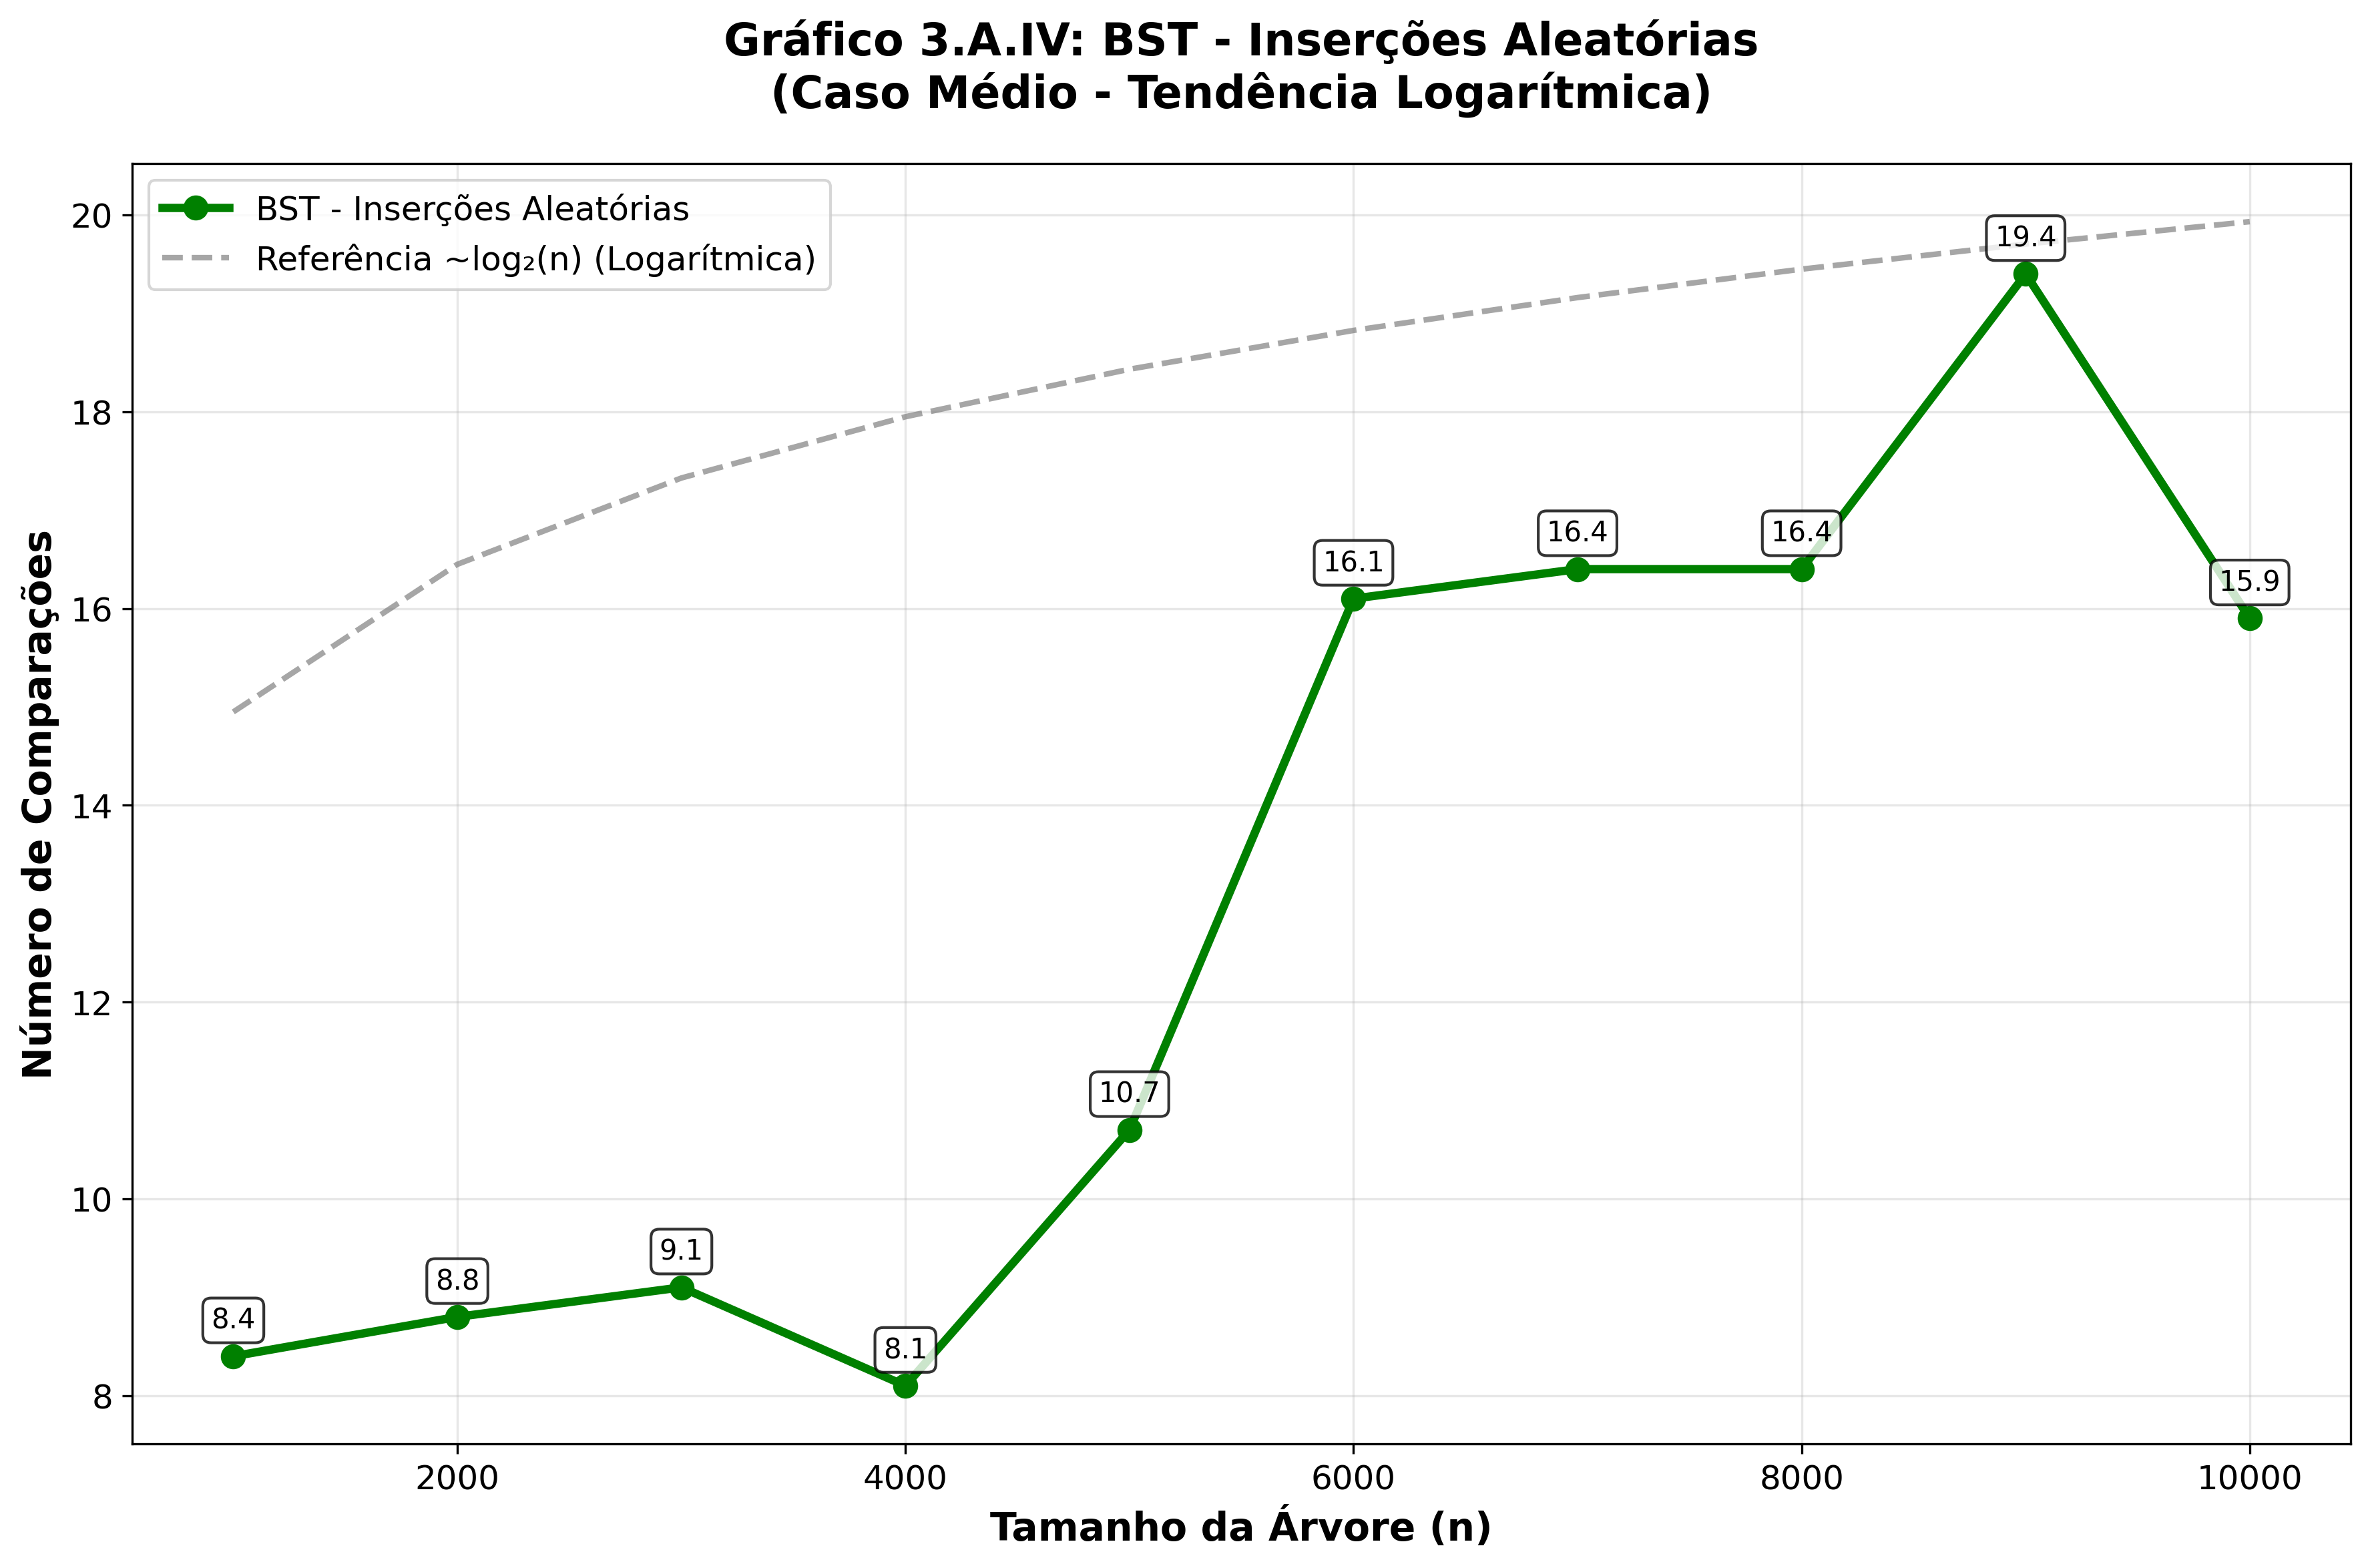
\includegraphics[width=0.8\textwidth]{graficos/grafico_3A_IV_bst_aleatorios.png}
    \caption{Gráfico 3.A.IV: BST - Inserções Aleatórias (Caso Médio - Tendência Logarítmica)}
    \label{fig:bst_aleatorios}
\end{figure}
Como podemos ver no gráfico da Figura~\ref{fig:bst_aleatorios}, quando os dados entram de forma aleatória, a BST se sai muito melhor. O número de comparações cresce devagar, seguindo uma curva logarítmica. Ou seja, a busca continua rápida mesmo com árvores grandes, desde que os dados não estejam em ordem. Isso mostra que a aleatoriedade ajuda a manter a árvore mais equilibrada, tornando as buscas eficientes.

\subsection*{AVL com Inserções Ordenadas}
\begin{figure}[H]
    \centering
    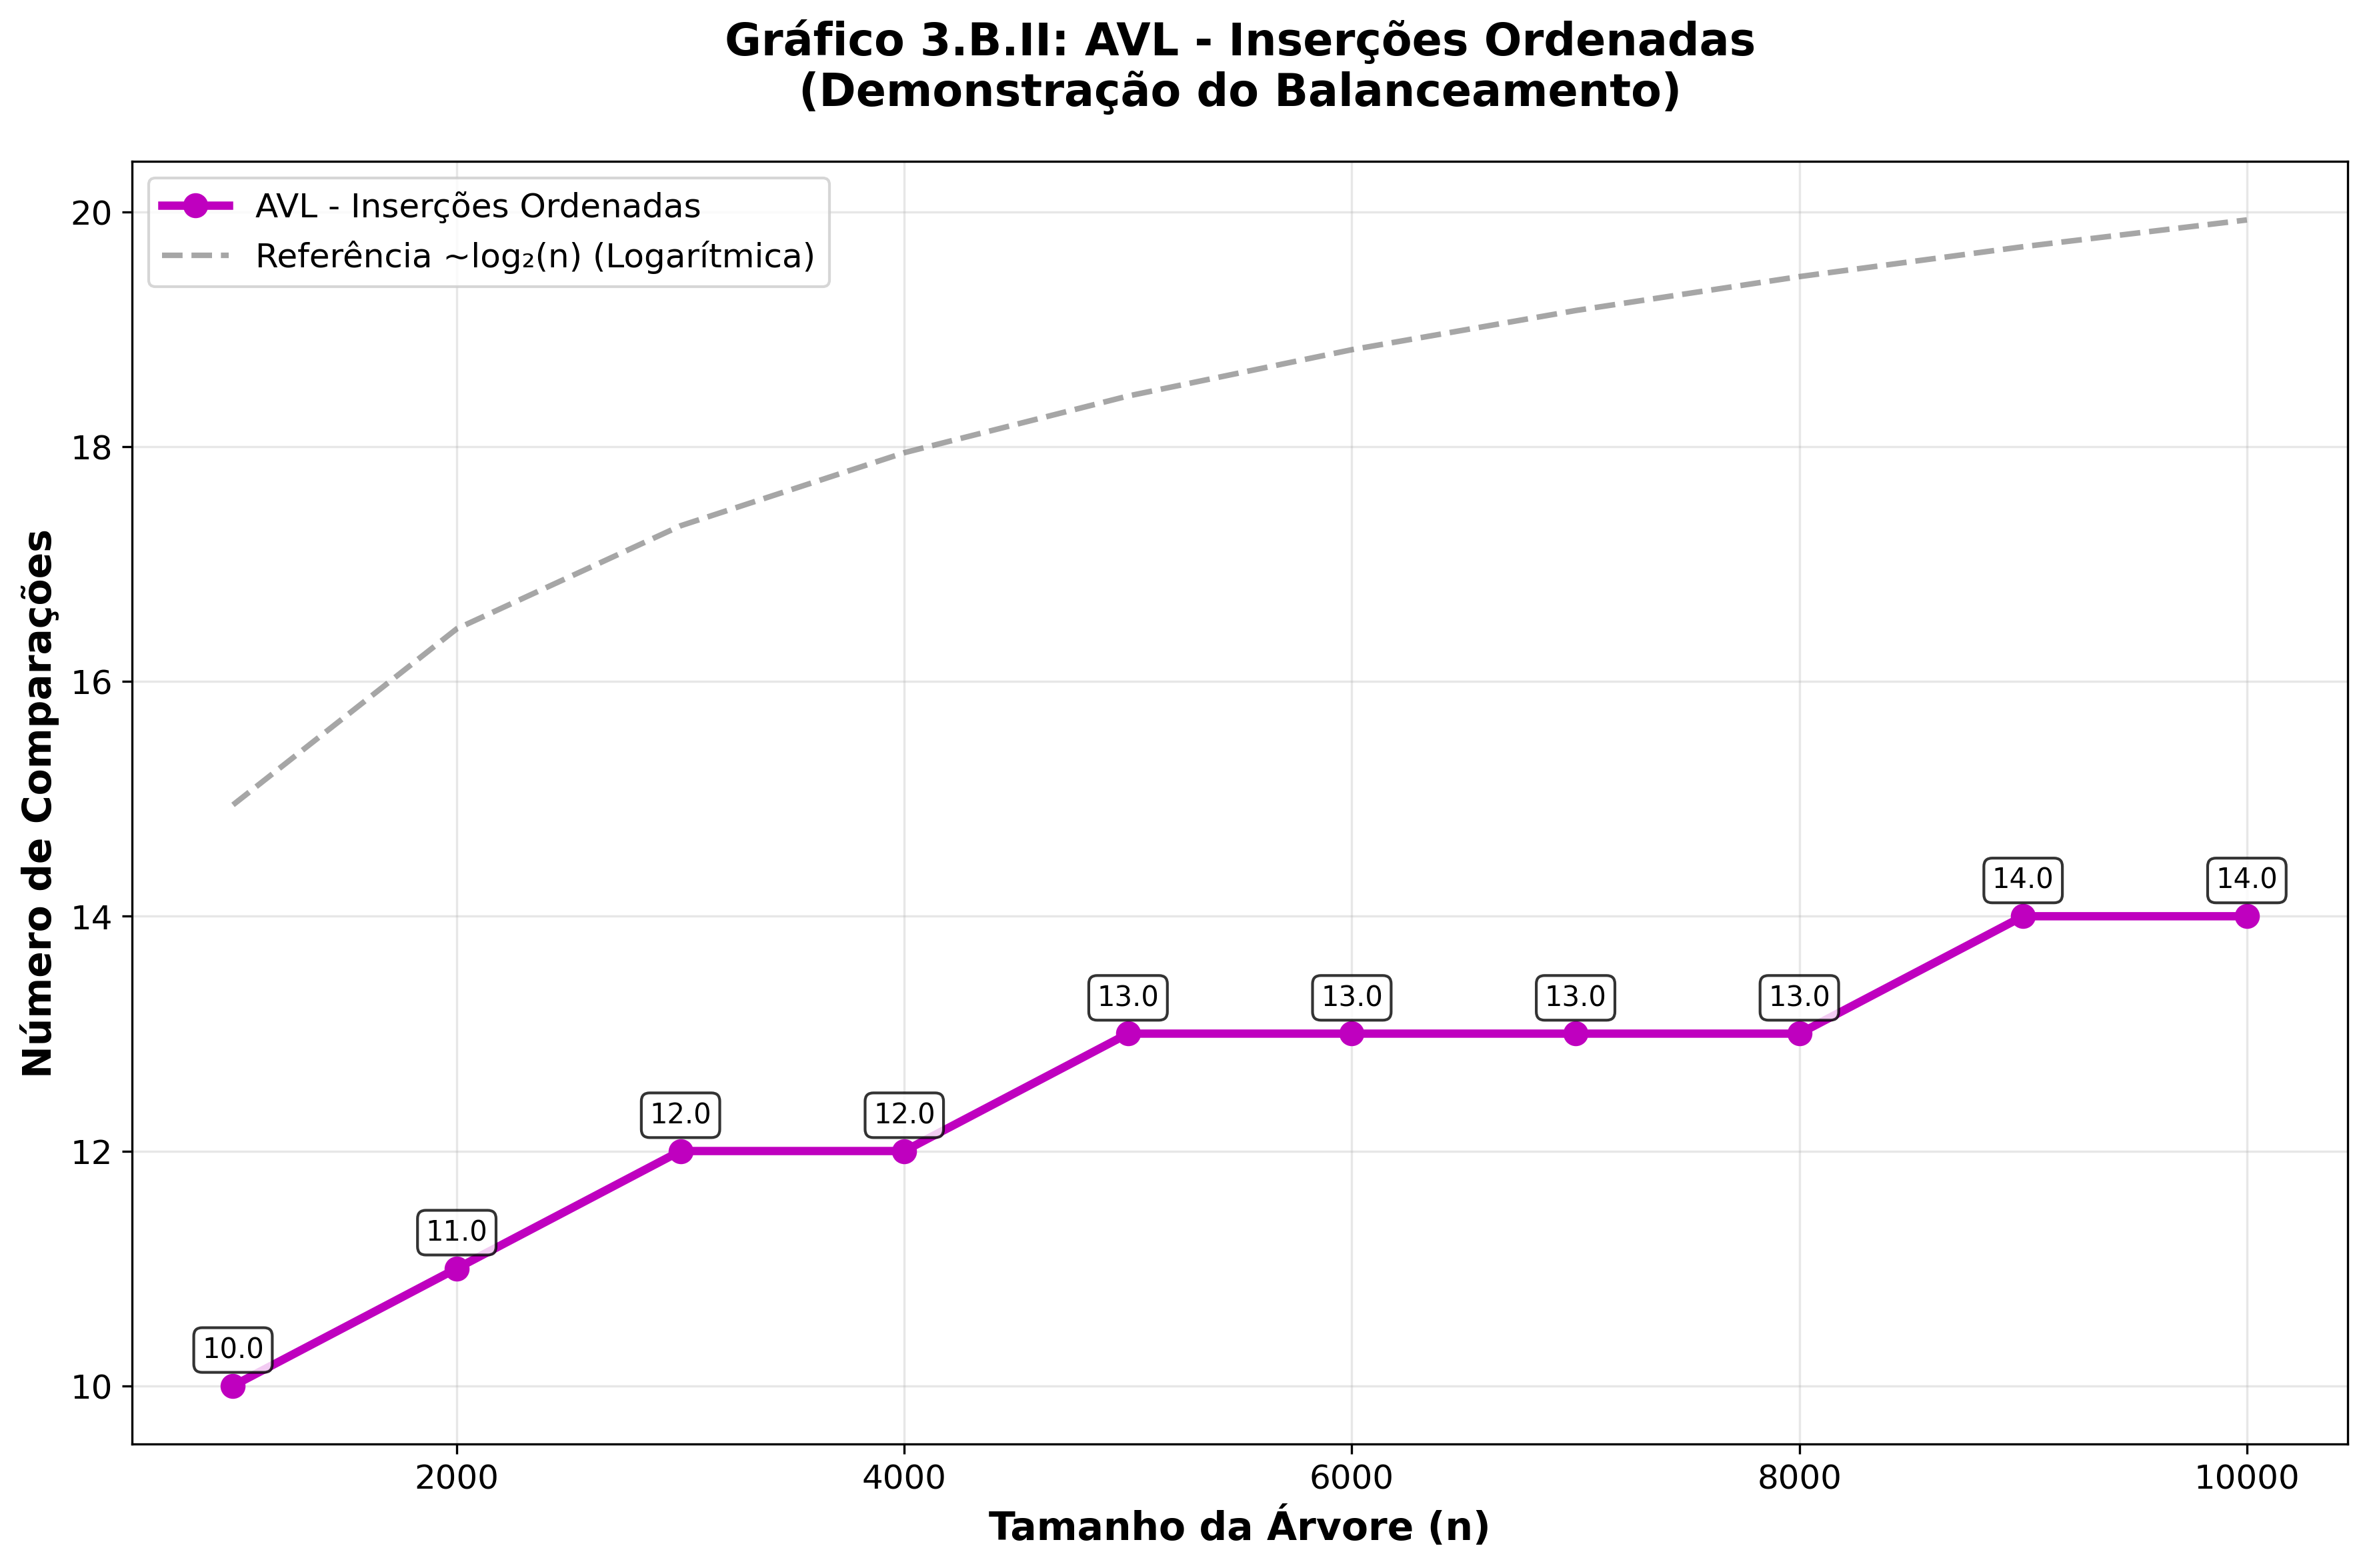
\includegraphics[width=0.8\textwidth]{graficos/grafico_3B_II_avl_ordenados.png}
    \caption{Gráfico 3.B.II: AVL - Inserções Ordenadas (Demonstração do Balanceamento)}
    \label{fig:avl_ordenados}
\end{figure}
Como podemos ver no gráfico da Figura~\ref{fig:avl_ordenados}, mesmo com dados em ordem, a AVL se ajusta automaticamente. O número de comparações cresce bem devagar, porque a árvore nunca vira "escada". O balanceamento garante que a busca seja sempre eficiente, independentemente da ordem dos dados inseridos. Isso mostra a vantagem do balanceamento automático da AVL.

\subsection*{AVL com Inserções Aleatórias}
\begin{figure}[H]
    \centering
    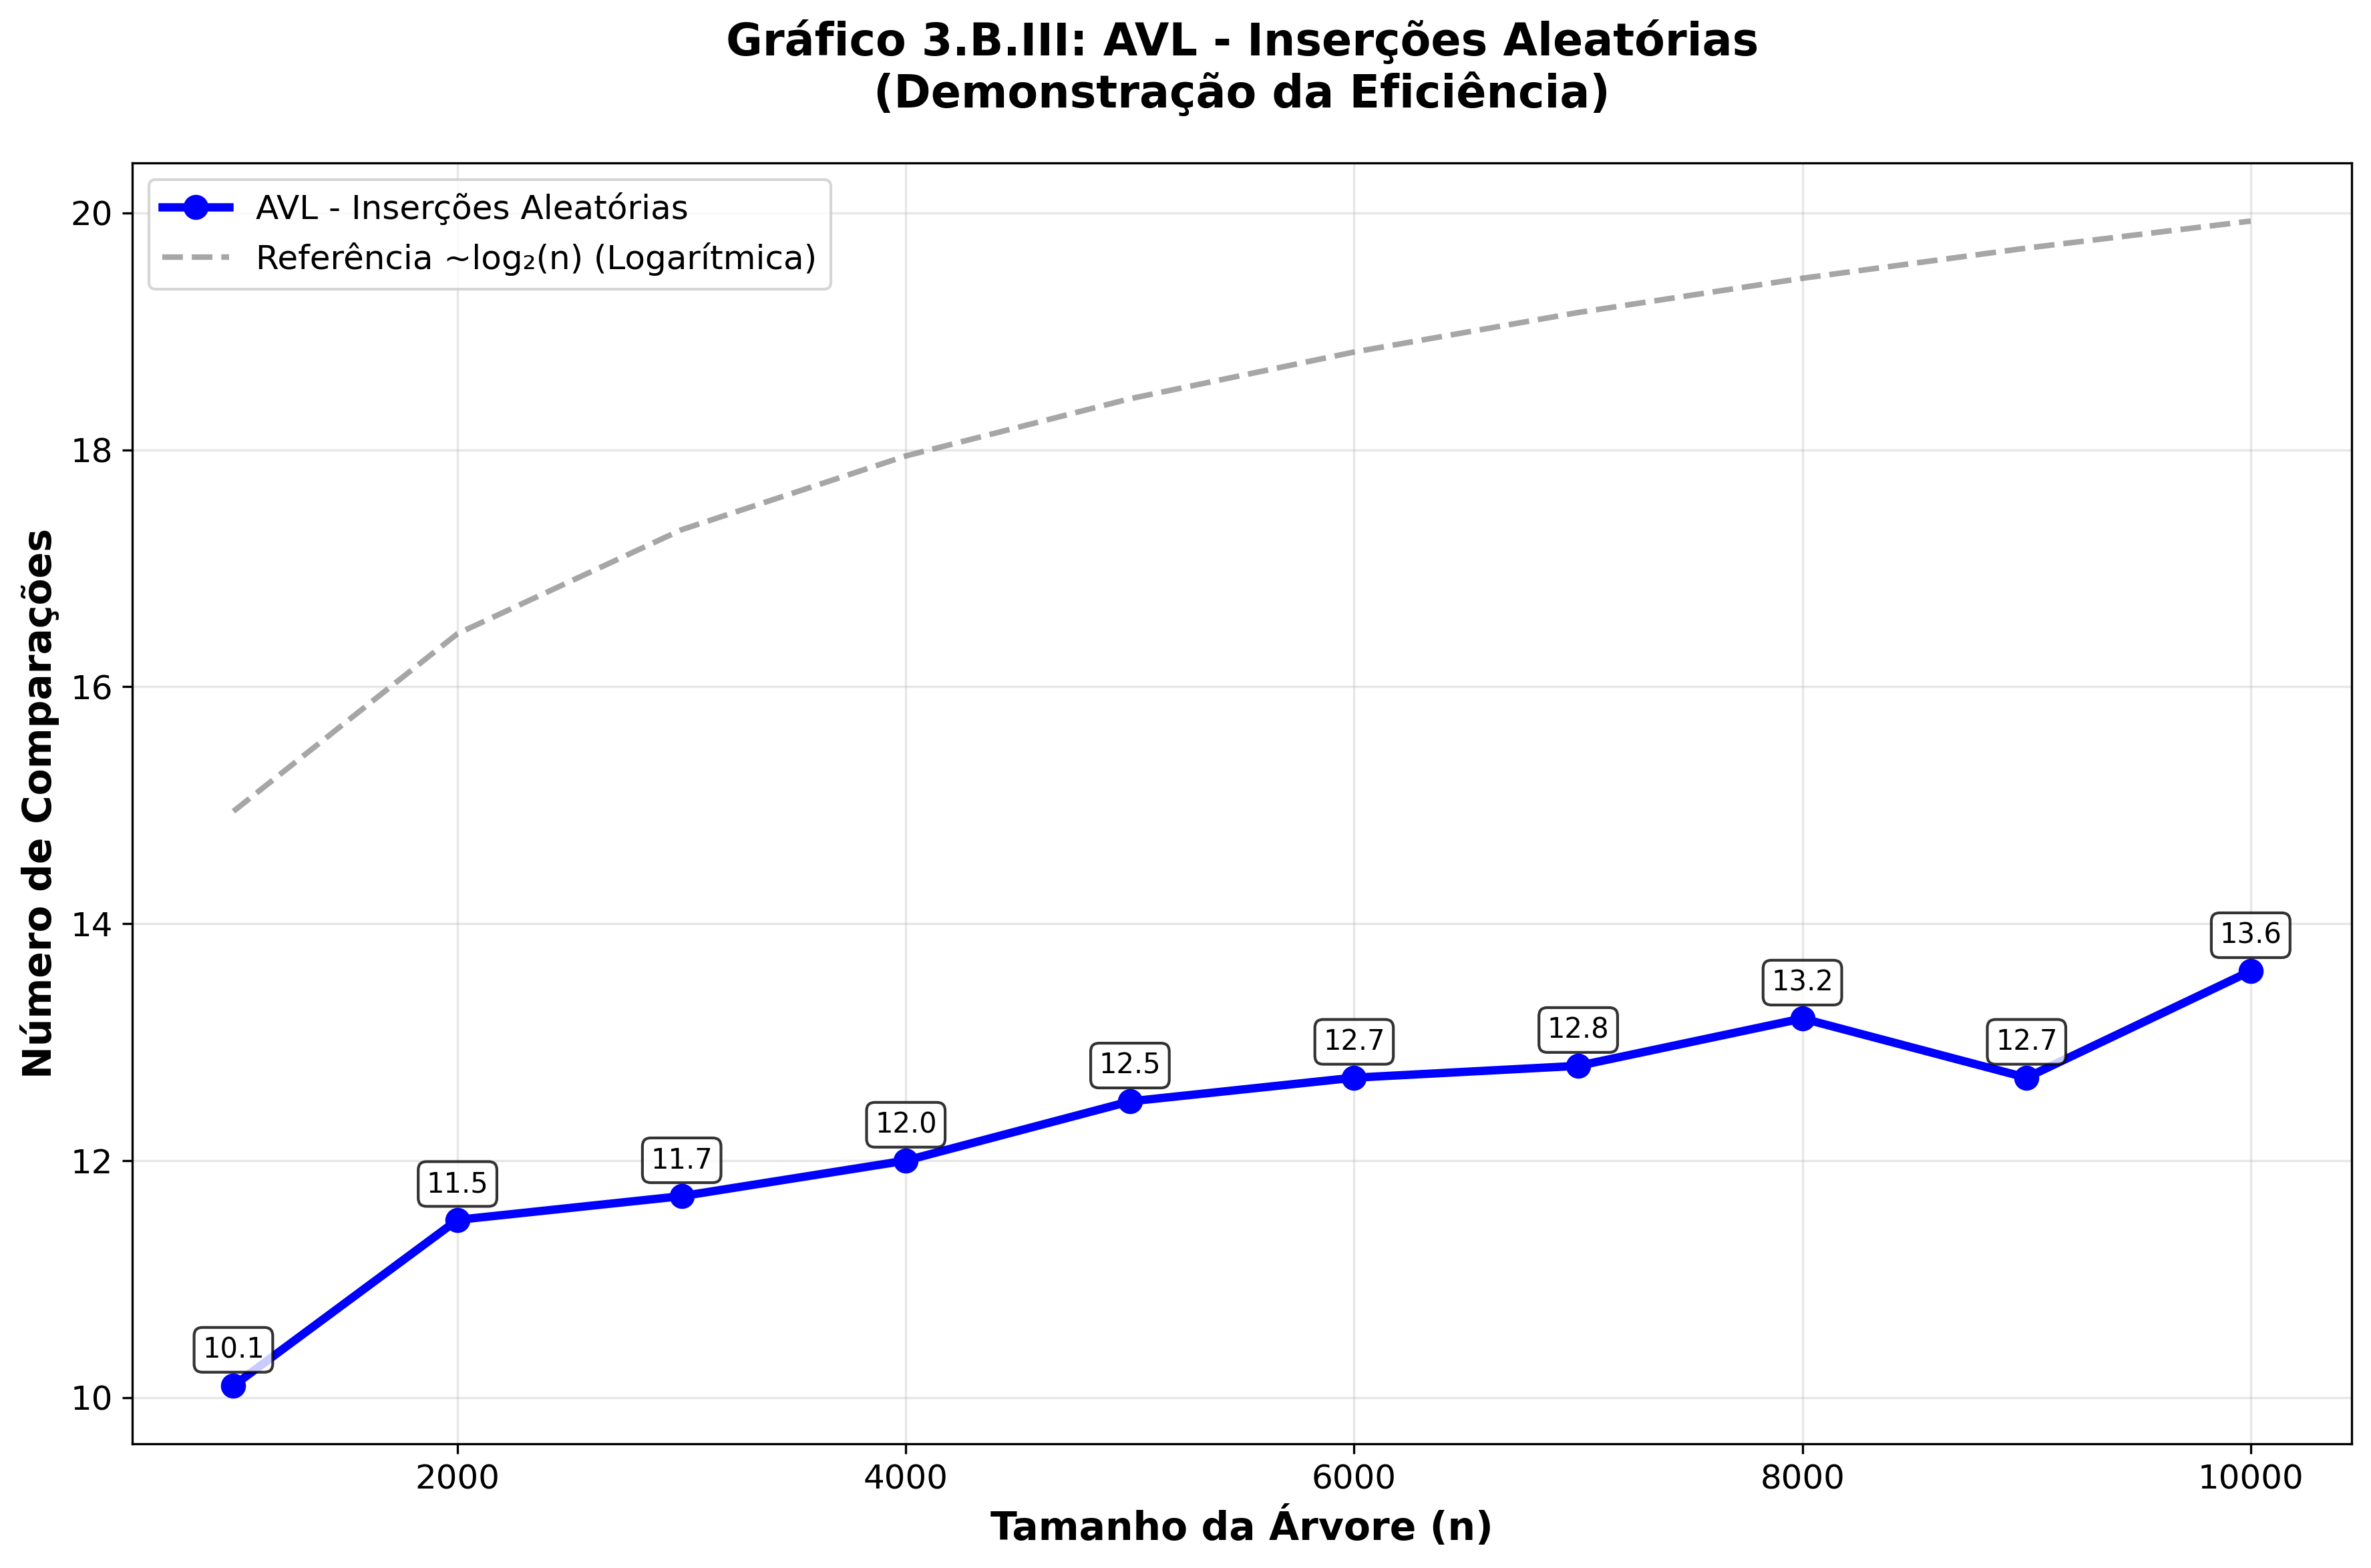
\includegraphics[width=0.8\textwidth]{graficos/grafico_3B_III_avl_aleatorios.png}
    \caption{Gráfico 3.B.III: AVL - Inserções Aleatórias (Demonstração da Eficiência)}
    \label{fig:avl_aleatorios}
\end{figure}
Como podemos ver no gráfico da Figura~\ref{fig:avl_aleatorios}, a AVL mantém a eficiência mesmo com dados aleatórios. O número de comparações fica sempre baixo, mostrando que o balanceamento automático funciona em qualquer situação. Por isso, a AVL é uma ótima escolha quando precisamos garantir buscas rápidas, não importa como os dados chegam. A estrutura se adapta e mantém a busca eficiente.


Os resultados evidenciam as diferenças de complexidade entre as estruturas:
\begin{itemize}
    \item \textbf{BST Ordenada}: Complexidade O(n) --- busca percorre todos os nós, desempenho insatisfatório em dados sequenciais.
    \item \textbf{BST Aleatória}: Complexidade O(log n) no caso médio --- árvore tende a ser mais balanceada, mas sem garantias absolutas.
    \item \textbf{AVL (Ordenada e Aleatória)}: Complexidade O(log n) garantida --- balanceamento automático impede degeneração e garante eficiência.
\end{itemize}

A AVL se destaca por garantir desempenho previsível e eficiente, enquanto a BST depende fortemente do padrão de inserção dos dados. O balanceamento automático é fundamental para aplicações que exigem performance consistente.

\section{Conclusão}



A Tabela~\ref{tab:media_comparacoes} apresenta as médias reais de comparações encontradas nos experimentos para cada estrutura e cenário testado. Fica evidente que a AVL mantém a eficiência em qualquer situação, enquanto a BST só é eficiente com dados aleatórios e perde desempenho drasticamente com inserções ordenadas. Os valores refletem o comportamento prático observado nos gráficos e análises do relatório.

\begin{table}[H]
    \centering
    \caption{Média das comparações encontradas nos experimentos}
    \begin{tabular}{lcc}
        \toprule
        \textbf{Estrutura} & \textbf{Inserção Aleatória} & \textbf{Inserção Ordenada} \\
        \midrule
        \textbf{BST} & 13 & 5500 \\
        \textbf{AVL} & 12 & 12 \\
        \bottomrule
    \end{tabular}
    \label{tab:media_comparacoes}
\end{table}



O objetivo deste trabalho foi comparar, de forma prática e didática, o desempenho das árvores binárias de pesquisa (BST) e das árvores AVL em operações de busca, considerando diferentes padrões de inserção de dados.

Os resultados mostram que a BST apresenta comportamento logarítmico e eficiência apenas com inserções aleatórias, mas degenera em uma lista ligada e perde desempenho com dados ordenados (média de 5500 comparações). Já a AVL mantém comportamento logarítmico e eficiência em todos os cenários, com médias próximas de 12 comparações, independentemente do padrão de inserção. Esses achados reforçam a importância do balanceamento automático para garantir buscas rápidas e previsíveis em grandes volumes de dados.

\begin{table}[H]
    \centering
    \caption{Comparação entre BST e AVL nos cenários testados}
    \begin{tabular}{lcc}
            \toprule
            \textbf{Estrutura} & \textbf{Inserção Aleatória} & \textbf{Inserção Ordenada}
        \\ \midrule
        BST & O(log n) & O(n)
        \\ AVL & O(log n) & O(log n)
        \\ \bottomrule
    \end{tabular}
    \label{tab:comparacao_bst_avl}
\end{table}


A Tabela~\ref{tab:comparacao_bst_avl} resume as complexidades teóricas observadas nos experimentos. Ela mostra que a AVL mantém buscas rápidas independentemente do padrão de inserção, enquanto a BST só é eficiente com dados aleatórios. Esses resultados reforçam que o balanceamento é fundamental para garantir buscas rápidas e previsíveis, especialmente em grandes volumes de dados. A AVL se mostrou superior à BST em todos os cenários, validando na prática os conceitos teóricos discutidos ao longo do trabalho.

\newpage
\bibliographystyle{abnt}
\begin{thebibliography}{99}

\bibitem{cormen2009}
CORMEN, T. H.; LEISERSON, C. E.; RIVEST, R. L.; STEIN, C. 
Algoritmos: Teoria e Prática. 3. ed. Rio de Janeiro: Elsevier, 2009. 

\end{thebibliography}

\end{document}
